\chapter{Background}
\label{background}

The goal of the proposed method is to include volumetric representations into a global illumination algorithm in a fast and coherent way. One of the unique features of participating media is that they must be represented with a more complex data-structure than solid geometric objects which are usually polygonalized in most rendering processes.  Light interacts with the particles of a volume, creating complex radiance patterns (increasing the necessary computational complexity exponentially.) In particular the most fundamental concepts are presented here,  (based off of  \cite{pbrt}).

%----------------------------------%
\section{Radiance}

\begin{figure}[h!]
    \centering
    \includegraphics[width=80mm]{../img/radiance.pdf}
    \captionfonts
    \caption{Evaluation of radiance at a point on an opaque surface.  Only the hemisphere around the surface normal is considered.  Incoming radiance is measured and scaled by its solid angle.}
    \label{fig:radiance}
\end{figure}

Irradiance is the change of flux (radiant power) over an area, denoted by $E = \frac{d\Phi}{dA}$ \cite{aga}. Another way to look at this problem involves the relationship between the surface and surrounding radiometric quantities.  Radiance helps us evaluate how much power enters or leaves any given point.  The definition of radiance leaving a surface can be denoted $L(\textup{p}, w)$ given $\textup{p}$ is the point on a surface and $w$ is the direction we are evaluating.  The flux is projected upon the area of the surface $dA$ based on the solid angle $dw$, which gives us Figure \ref{fig:radiance} and the following equation:

\begin{equation}
\mathit{L} = \frac{\mathit{d^{2}\Phi}}{\mathit{dwdA}^\perp}
\label{eq:radiance}
\end{equation}

Inversely, incoming radiance, or irradiance, is evaluated by the strength of the light coming from any given direction $w$.  This  can be represented by the following:

\begin{equation}
\mathit{E} = \int\mathit{L}(\textup{p} \leftarrow w)\textup{cos}\theta dw.
\label{eq:irradiance}
\end{equation}

$\mathit{L}(\textup{p} \to w)$ represents the radiance leaving point $\textup{p}$ and $\mathit{L}(\textup{p} \leftarrow w)$ represents incoming radiance given a direction $w$.  Note that radiance along a straight path is invariant.  For example:

\begin{equation}
L(x \to y) = L(y \to x).
\label{eq:invariance}
\end{equation}

Measuring the incoming radiance at any given point $\textup{p}$ in all directions is the key to the graphics lighting equation, and a crucial element in how a rendered scene looks and feels.

\section{BRDF and the BSSRDF}

The \textit{bidirectional reflectance distribution function} (or BRDF) is a function that gives us a formal method of describing the reflected radiance from a surface based on incident radiance from another light source or emissive surface \cite{pbrt}.  This simplification helps us with quick evaluations in scenes with simple lighting (such as point light sources) and other direct-lighting techniques.  First, let us consider the formalization of irradiance we discussed earlier by defining the following equation:

\begin{equation}
\textup{d}\mathit{E}(\textup{p}, w_{i}) = \mathit{L}_{i}(\textup{p}, w_{i})\textup{cos}\theta_{i} \textup{d}\mathit{w_{i}}.
\label{eq:brdf_irrid}
\end{equation}

Using Equation \ref{eq:brdf_irrid}, can create a proportionality of light reflected from point p towards outgoing direction $w_o$ due to incoming light from incident direction $w_i$, giving us the following equation:

\begin{equation}
f_r(\textup{p}, w_o, w_i) =  \frac{dL_o(\textup{p},w_o)}{dE(\textup{p},w_i)}.
\label{eq:brdf_func}
\end{equation}

In traditional three-dimensional scene descriptions we are given a distribution to replace Equation \ref{eq:brdf_func}, allowing us to solve for $L_o$, our outgoing radiance.  This leaves us with:

\begin{equation}
\mathit{L_o}(\textup{p}, w_o) = \int_{\mathbb{S}^2} \mathit{f_r}(\textup{p}, w_o, w_i)\:L_i(\textup{p}, w_i)cos\theta_i dw.
\label{eq:brdf_solve}
\end{equation}


Many materials such as skin, marble and plastic do not simply reflect the incoming light energy, but also transmit it through the surface, a process called \textit{subsurface scattering}.  Given the obvious shortfalls of the BRDF in this instance, the BSSRDF (\textit{bidirectional scattering-surface reflectance distribution function}) takes into account a surface's scatter properties.  This generalized function describes the ratio of radiance from an incoming point and direction $\textit{p}_{i}$, $w_{i}$ to an outgoing point and direction $\textit{p}_{i}$, $w_{o}$.  The following describes the new proportionality created from the BSSRDF:

\begin{equation}
f_r(\textup{p}_o, w_o, \textup{p}_i, w_i) =  \frac{dL_o(\textup{p}_o,w_o)}{dE(\textup{p}_i,w_i)}.
\label{eq:brdf_bssrdf}
\end{equation}

If we were to use Equation \ref{eq:brdf_bssrdf}, we would be able to iterate over every incoming point and every incoming direction in order to evaluate the outgoing radiance at an arbitrary point, turning a one-dimensional reflectance equation into a two-dimensional scatter equation and significantly increasing its complexity.

\section{Volume Lighting}

The BSSRDF describes the complexities of light traveling and scattering within complex surfaces similarly to that of volumes.  Volumes follow very similar behaviors to opaque surfaces in terms of radiance, except on a particle-level.  Participating media like smoke or fog is made up of particles which cause the scatter (i.e. clouds) and absorption/extinction (i.e. smoke,) behaviors that would be extremely computationally expensive to model and simulate on any scale.  Therefore, such behaviors are modeled in terms of transmittance, emission, Scatter in and Scatter out like in Figure \ref{fig:vol_scat}.  We are able to identify the probability that light will be absorbed, scattered and/or transmitted through any point in a participating medium by identifying their probability density functions, as described in the following sections. 
\begin{figure}[h!]
    \centering
    \includegraphics[width=100mm]{../img/vol_scatter.pdf}
    \captionfonts
    \caption{Light scatter properties vary based on the participating media.}
    \label{fig:vol_scat}
\end{figure}

%----------------------------------%
\subsection{Absorption:}
As light passes through a participating media, light will become absorbed based on its absorption probability density $\sigma_{a}$. As stated earlier in Equation \ref{eq:invariance}, it is known that radiance along a straight path is invariant, which allows us to estimate the amount of light absorbed or scattered given point $p$ and direction $w$ with the following:

\begin{equation}
e^{-\int_{0}^{d}\sigma_{a} (p+t\mathit{w},\mathit{w})d\mathit{t}},
\label{siga_eq}
\end{equation}

where $\sigma_{a}$ represents the probability density that light will be absorbed over a distance $\textup{d}\mathit{t}$.

%----------------------------------%
\subsection{Scatter Out:}
In addition to being absorbed by the medium, light can be scattered based on a scatter probability density $\sigma_{s}$.  As light is scattered and thus redirected, the amount of energy passing through the density in direction $w$ is reduced.  We can model the scatter equation through the following equation:

\begin{equation}
\textup{d}\mathit{L}_{o}(\textup{p},w) = -\sigma_{s}(\textup{p},w) \mathit{L}_{i}(\textup{p},-w)\textup{d}t.
\label{sigs_eq}
\end{equation}

$\textup{d}L_{o}$ represents the outgoing radiance given point $\textup{p}$ and direction $w$.

%----------------------------------%
\subsection{Transmittance:}
Both Equation (\ref{siga_eq}) and Equation (\ref{sigs_eq}) involve the reduction of energy through a volume, reducing how much energy passes through (also known as its transmittance.)  The two can be combined into the following overarching representation:

\begin{equation}
\sigma_{t}(\textup{p},w) = \sigma_{a}(\textup{p},w) + \sigma_{s}(\textup{p}, w).
\label{eq:sigt}
\end{equation}

Equation \ref{eq:sigt} gives us transmittance ($\sigma_{t}$) at point $\textup{p}$ and direction $w$.  Using this representation, we can integrate over a ray passing through the volume in order to evaluate the resulting radiance transmittion:

\begin{equation}
T_{r}(\textup{p} \to \textup{p}') = e^{-\int_{0}^{d}\sigma (p+t\mathit{w},\mathit{w})d\mathit{t}}.
\label{transmittion_eq}
\end{equation}

%----------------------------------%
\subsection{Phase Functions}

\begin{figure}[h!]
    \centering
    \includegraphics[width=80mm]{../img/phase_func.pdf}
    \captionfonts
    \caption{Visual representation of a phase function around a scatter point.  The area represents the distribution of the scattered light about a sphere.}
    \label{fig:phase}
\end{figure}

When dealing with particles in volumes that may scatter light, a distribution function or \textit{phase function} describes the angular distribution of light scattered, described as $phase(w \to w')$.  The probability that light may scatter from direction $w$ to $w'$ is described using this function.  This distribution is visualized in Figure \ref{fig:phase}. All tests in this paper were rendered using one of the simplest phase functions, known as the isotropic or \textit{constant} phase function which represents the BRDF analog for participating media \cite{cerezo}.


%----------------------------------%
\subsection{Scatter In}
Although $\sigma_{s}$ may contribute to light being scattered out (and reduce the energy of a ray passing through the volume,) radiance from other rays (scattered by their respective phase functions as seen in Figure \ref{fig:phase}) may contribute to the original ray's radiance.  This allows for radiance emitted from surrounding participating media and geometry to contribute to the light we are sampling through the volume, as exemplified in Figure \ref{fig:inscat_comp}.  Before we can integrate incoming radiance, we must guarentee that the phase function represents a normalized distribution, where the following constraint must hold true:

\begin{equation}
\int_{\mathbb{S}^2}phase(w \to w')\textup{d}w' = 1.
\label{eq:source}
\end{equation}

This normalization forces the phase function to accurately define the probability distribution for a particular direction.  Given a summation of all outgoing radiance along every direction $w'$, we should be left with the total incoming radiance from direction $w$.

\begin{figure}[h!]
    \centering
    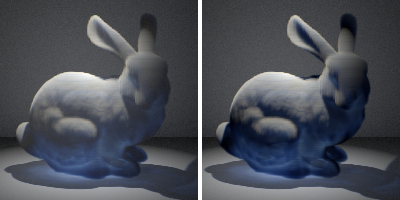
\includegraphics[width=80mm]{../img/inscat_comp.png}
    \captionfonts
    \caption{Comparison between a volume with (right) and without (left) in-scattering contribution.}
    \label{fig:inscat_comp}
\end{figure}

Finally, assuming conditions are met for Equation \ref{eq:source}, we can integrate the total radiance scatter based on the normalized phase function $phase(w \to w')$ over all directions $w'$ to get our total scatter in a direction $w$:

\begin{equation}
\mathit{S}(\textup{p},w) = \mathit{L}_{\textup{ve}}(\textup{p},w) + \sigma_{\textup{s}}(\textup{p}, w) \int_{\mathbb{S}^2} phase(\textup{p}, -w' \to w) L_{i}(\textup{p},w')\textup{d}w'.
\label{eq:scat_in}
\end{equation}

$L_{\textup{ve}}(\textup{p}, w)$ represents the emission coefficient of a volume and is not discussed in this paper.

When we integrate over the domain of the sphere in Equation \ref{eq:scat_in}, we are essentially testing for the incoming light in every direction, testing how much light from that incoming direction scatters towards our ray, and accumulate that light until we have all of the light contributing to this particular ray.


\section{Monte Carlo Integration}

Monte Carlo methods have many applications in estimating complex systems through the use of random numbers and sampling schemes.  One of the most useful technique is Monte Carlo integration, which estimates the integral of an arbitrary function through sampling discrete values defined over a specified domain \cite{aga}.  For this reason, Monte Carlo has become \textit{integral} in the field of computer graphics, where it may manifest itself in evaluating incoming radiance over a surface, estimating light scatter, or randomly sampling area lights in order to get soft shadows.

Many of the elements listed above can be (and are) estimated using this technique.  In order to get good results, however, many hundreds of samples may be necessary.  The cost of sampling using this method may still be cost-prohibitive, at which point the problem lies in the sample method itself, not how the samples are used or generated.

